\label{impl_exp}

\subsection{RMSD Benchmark}
\label{sec:RMSD}
The RMSD algorithm represents a task whose computational load is smaller than the I/O load per frame (typical values $t_{\text{compute}}^{\text{frame}} = 0.09\ \text{ms}$, $t_{\text{IO}}^{\text{frame}} = 0.3\ \text{ms}$, thus $\overline{\tcomp}/\overline{\tIO} \approx 0.3$). 
We showed in~\cite{Khoshlessan:2017ab} that the RMSD task only scaled well up \gpnote{I removed the number of cores because Stampede had 16 cores and Comet has 24}on a single compute node on \emph{SDSC Comet}, and \emph{TACC Stampede}, using either Dask or MPI.

We focus on the MPI implementation (via \package{mpi4py}~\cite{Dalcin:2011aa, Dalcin:2005aa}) to better understand the cause for the lack of scaling across nodes.
As in our previous work, we also observed very poor strong scaling performance (Figures~\ref{fig:MPIscaling},~\ref{fig:MPIspeedup} and~\ref{fig:MPIscaling-Bridges} and~\ref{fig:MPIspeedup-Bridges}) beyond a single node.
A more detailed analysis showed that the RMSD computation, and to a lesser degree the I/O, considered on their own scaled well beyond 50 cores (yellow and blue lines in Figure~\ref{fig:ScalingComputeIO}). 
But, communication (red line in Figure~\ref{fig:ScalingComputeIO}) and the initial file opening (gray line in Figure~\ref{fig:ScalingComputeIO}) started to dominate beyond 50 cores.
Communication cost and initial time for opening the trajectory were distributed unevenly across MPI ranks, as shown in Figure~\ref{fig:MPIranks}. 
The ranks that took much longer to complete than the typical execution time of the other ranks were the stragglers that hurt performance.

\subsubsection*{Identification of Scalability Bottlenecks}
In the example shown in Figure~\ref{fig:MPIranks}, 62 ranks out of 72 took about $60sec$ (the stragglers) whereas the remaining ranks only took about $20sec$. 
The detailed breakdown of the time spent on each rank (Figure~\ref{fig:MPIranks}) showed that the computation, \tcomp, was relatively constant across ranks. 
The time spent on reading data from the shared trajectory file on Lustre into memory, \tIO, showed variability across different ranks. 
The stragglers, however, appeared to be defined by occasionally much larger \emph{communication} times, \tcomm (line 16 in Algorithm~\ref{alg:RMSD}), which were on the order of $30sec$, and by larger times to initially open the trajectory (line 2 in Algorithm~\ref{alg:RMSD}).
\tcomm varied across different ranks and was barely measurable for a few of them.
Although the data in Figure~\ref{fig:MPIranks} represent one run and in other instances different number of ranks were stragglers, the overall hypothesis was confirmed by the averages over five independent repeats and all ranks (Figure~\ref{fig:ScalingComputeIO}).
This initial analysis indicated that communication was a major issue that prevented good scaling beyond a single node but the problems related to file I/O also played an important role in limiting performance.

\begin{figure}
\centering
\begin{subfigure}{.4\textwidth}
  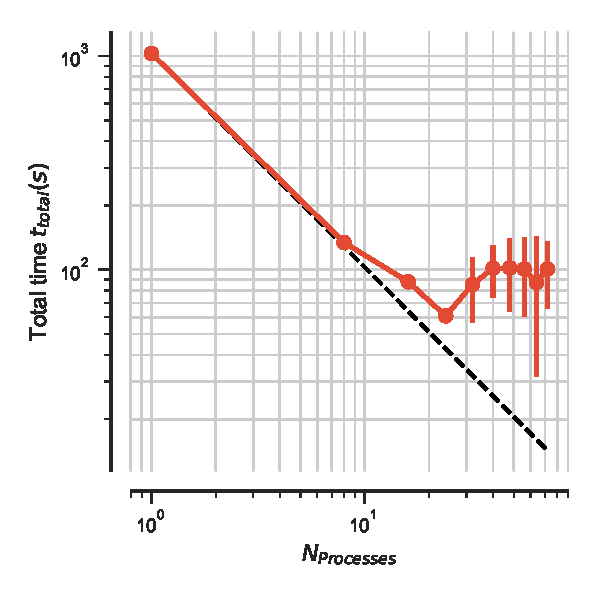
\includegraphics[width=\linewidth]{figures/main-RMSD-t_total.pdf}
  \captionsetup{format=hang}
  \caption{Scaling total (five repeats)}
  \label{fig:MPIscaling}
\end{subfigure}
\hfill
\begin{subfigure}{.4\textwidth}
  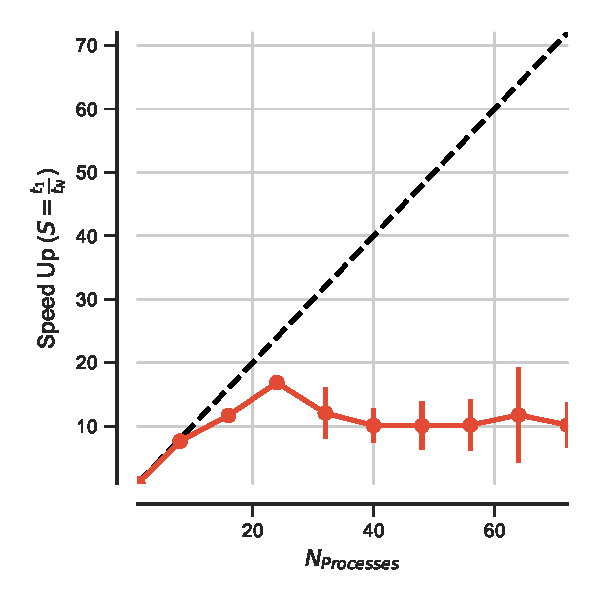
\includegraphics[width=\linewidth]{figures/main-RMSD-speed_up.pdf}
  \captionsetup{format=hang}
  \caption{Speed-up (five repeats)}
  \label{fig:MPIspeedup}
\end{subfigure}
\bigskip

\begin{subfigure}{.4\textwidth}
  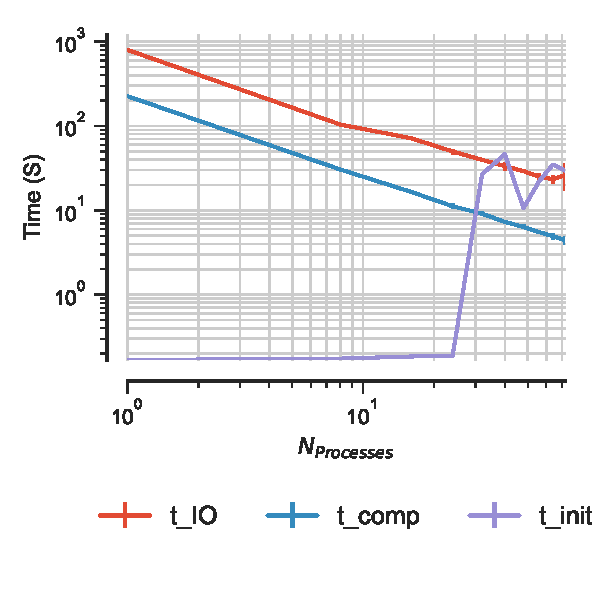
\includegraphics[width=\linewidth]{figures/main-RMSD-time_comp_IO_comparison.pdf}
  \captionsetup{format=hang}
\caption{Scaling for different components (five repeats)}
\label{fig:ScalingComputeIO}
\end{subfigure}
\hfill
\begin{subfigure} {.5\textwidth}
  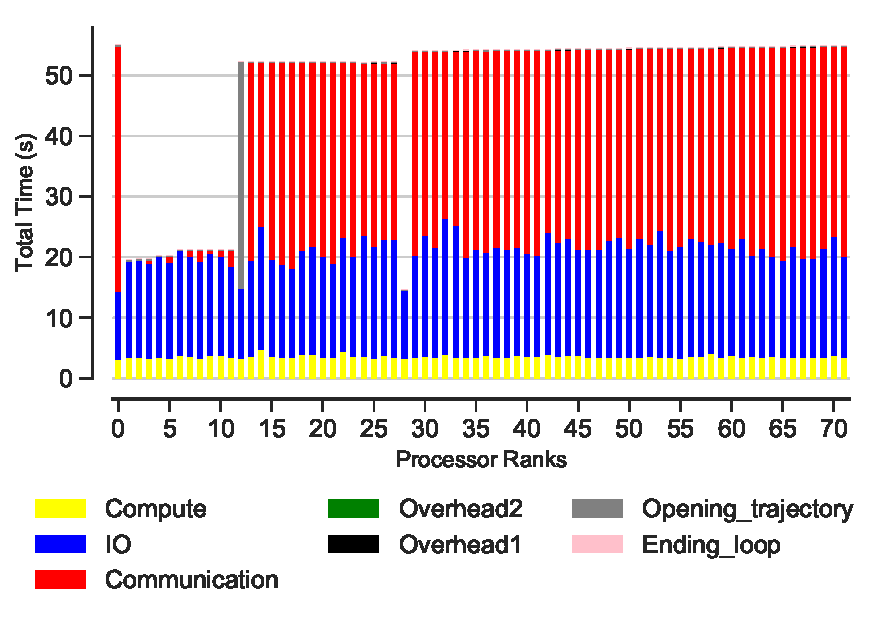
\includegraphics[width=\linewidth]{figures/main-RMSD-BarPlot-rank-comparison_72_5.pdf}
  \captionsetup{format=hang}
  \caption{Time comparison on different parts of the calculations per MPI rank (example)}
  \label{fig:MPIranks}
\end{subfigure}

\caption{Performance of the RMSD task (I/O-bound with $\overline{\tcomp}/\overline{\tIO} \approx 0.3$) with MPI on \emph{SDSC Comet}.
Results were communicated back to rank 0. Five independent repeats were performed to collect statistics. (a-c) The error bars show
standard deviation with respect to mean. (d) Compute \tcomp, IO \tIO, communication \tcomm, ending the for loop $t_{\text{end\_loop}}$,
  opening the trajectory $t_{\text{opening\_trajectory}}$, and overheads $t_{\text{overhead1}}$, $t_{\text{overhead2}}$ per MPI rank (see Table \ref{tab:notation} for the definition).
These are data from one run of the five repeats. MPI ranks 0, 12--27 and 29--72 are stragglers. \textbf{Note:} In serial, there is no communication.}
\label{fig:MPIwithIO}
\end{figure} 

\subsubsection*{Influence of Hardware}
We ran the same benchmarks on multiple HPC systems (XSEDE's \emph{PSC Bridges} (Fig.~\ref{fig:MPIwithIO-Bridges}) and \emph{LSU SuperMIC} (Fig.~\ref{fig:MPIwithIO-SuperMIC})), and observed the occurrence of stragglers, in a manner very similar to the results described for \emph{SDSC Comet}.
There was no clear pattern in which certain MPI ranks would always be a straggler, neither could we trace stragglers to specific cores or nodes.
Therefore, the phenomenon of stragglers in the RMSD case was reproducible on different clusters and thus appeared to be independent from the underlying hardware.

\subsection{Effect of average compute over average IO ratio on Performance}
\label{sec:bound}

The results in section~\ref{sec:RMSD} indicated communication and I/O to be two important factors that appeared to correlate with stragglers. 
In order to better characterize the RMSD task, we computed the ratio between the time to complete the computation and the time spent on I/O, $\overline{\tcomp}/\overline{\tIO} = 0.3$, and found that this task was I/O bound, i.e.,
\begin{gather*}
  \frac{\overline{\tcomp}}{\overline{\tIO}} \ll 1.
\end{gather*}

For such a I/O-bound task we were not able to achieve good scaling beyond a single node. 
We hypothesized that decreasing the relative I/O load with respect to the compute load would also reduce the impact of stragglers by interleaving I/O with longer periods of computation and thus reducing the impact of I/O contention.
We therefore set out to measure compute bound tasks, i.e.\ ones with
\begin{gather*}
  \frac{\overline{\tcomp}}{\overline{\tIO}} \gg 1.
\end{gather*}
To measure the effect of the $\overline{\tcomp}/\overline{\tIO}$ ratio on performance but leaving other parameters the same, we artificially increased the computational load by repeating the same RMSD calculation (line 10, algorithm \ref{alg:RMSD}) 40, 70 and 100 times in a loop, resulting in forty-fold (``$40\times$''), seventy-fold (``$70\times$''), and one hundred-fold (``$100\times$'') load increases.

\subsubsection{Effect of Increased Compute workload for RMSD Task}

The increased computational workloads corresponded to $\overline{\tcomp}/\overline{\tIO}$ ratios of 11, 19, 27 respectively as shown in Table \ref{tab:load-ratio}.
\gpnote{I am not sure if this breaking passes the same message. It needs fixing.}
In fact, the $\overline{\tcomp}/\overline{\tIO}$ ratio for the higher workloads (with factor $X$) should be $X$ times the $\overline{\tcomp}/\overline{\tIO}$ for the $1\times$ workload (in agreement with theoretical prediction in Table \ref{tab:load-ratio}).
This is since on average the I/O workload of each rank is $N_{\text{b}} \times \tIO $, which is independent of $X$. 
However, the workload for the computation is $X \times N_{\text{b}} \times \tcomp$, and hence the ratio is $X \times \overline{\tcomp}/\overline{\tIO}$.

\begin{table}[ht!]
\centering
\begin{tabular}{rrrrr}
  \toprule
  \bfseries\thead{Workload} &  \bfseries\thead{$\tcomp$} &  \bfseries\thead{$\tIO$}
  & \multicolumn{2}{c}{\bfseries\thead{$\overline{\tcomp}/\overline{\tIO}$}}\\
  & & & \thead{measured} & \thead{theoretical}\\
  \midrule
    $1\times$   &   226 & 791 &  0.29 &   \\  
    $40\times$  &  8655 & 791 & 11   & 11\\    
    $70\times$  & 15148 & 791 & 19   & 20\\  
    $100\times$ & 21639 & 791 & 27   & 29\\  
  \bottomrule
\end{tabular}
\caption[Change in load-ratio with RMSD workload]{Change in $\overline{\tcomp}/\overline{\tIO}$ ratio with change in the RMSD workload.
  The RMSD workload was artificially increased in order to examine the effect of compute to I/O ratio on the performance.
  The reported compute and I/O time were calculated based on the serial version using one core and used to calculate the measured $\overline{\tcomp}/\overline{\tIO}$.
  The theoretical $\overline{\tcomp}/\overline{\tIO}$ (see text) is provided for comparison.}
\label{tab:load-ratio}
\end{table}

We performed this experiment to show the effect of the $\overline{\tcomp}/\overline{\tIO}$ ratio on performance (Figure~\ref{fig:tcomp_tIO_effect}).
As the $\overline{\tcomp}/\overline{\tIO}$ ratio increased, speed-up and performance improved, and showed overall better scaling than the I/O-bound workload, i.e. $1\times$ RMSD (Figure~\ref{fig:S1_tcomp_tIO_effect}).
The RMSD calculation consistently scaled up to larger numbers of cores ($N=56$ for $70\times$ RMSD) for higher $\overline{\tcomp}/\overline{\tIO}$ ratios.
Figures \ref{fig:S2_tcomp_tIO_effect} and \ref{fig:E_tcomp_tIO_effect} show that speed-up and efficiency approach their ideal value for each processor count with increasing $\overline{\tcomp}/\overline{\tIO}$ ratio.

\begin{figure}[ht!]
\centering
\begin{subfigure} {.3\textwidth}
  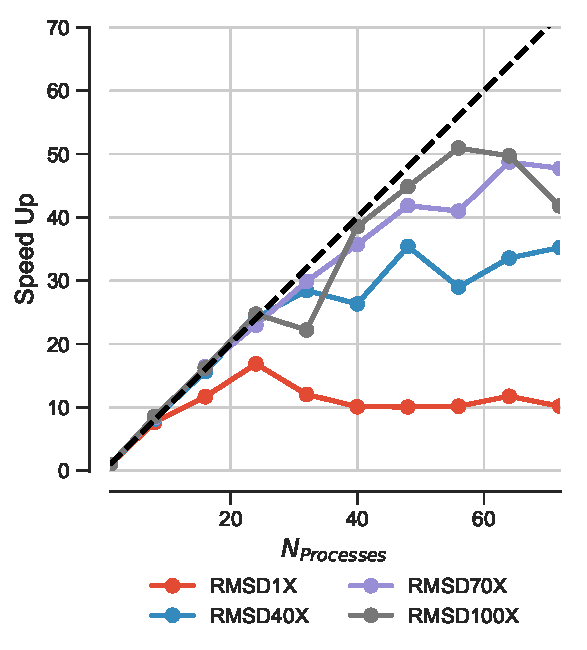
\includegraphics[width=\linewidth]{figures/Compute_to_IO_ratio_on_performance_2d_v17.pdf}
  \caption{Speed-Up}
  \label{fig:S1_tcomp_tIO_effect}
\end{subfigure}
\hfill
\begin{subfigure}{.3\textwidth}
  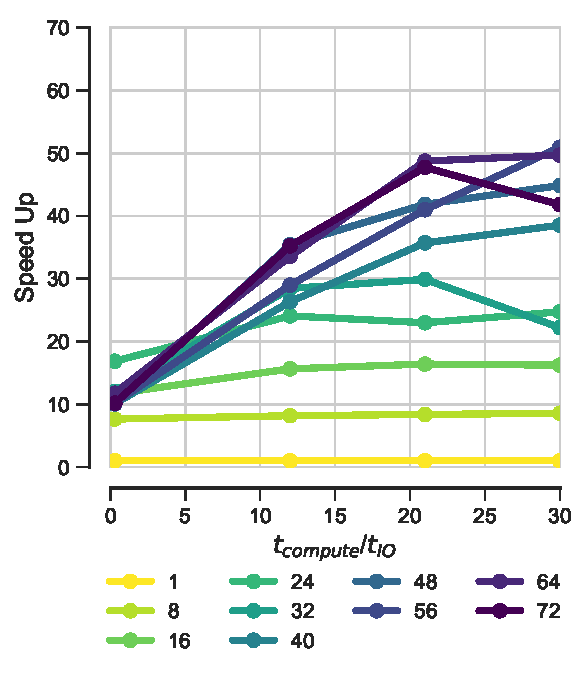
\includegraphics[width=\linewidth]{figures/Compute_to_IO_ratio_on_performance_2d_2_v17.pdf}
  \caption{Speed-Up}
  \label{fig:S2_tcomp_tIO_effect}
\end{subfigure}
\hfill
\begin{subfigure}{.3\textwidth}
  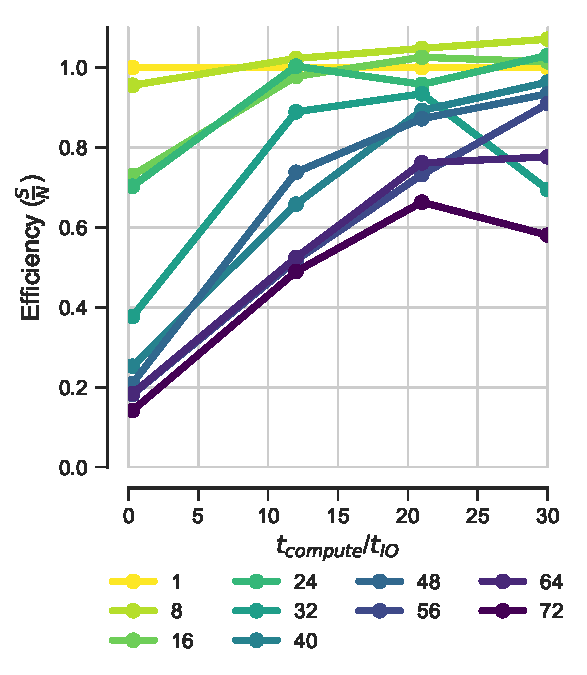
\includegraphics[width=\linewidth]{figures/Compute_to_IO_ratio_on_performance_2d_3_v17.pdf}
  \caption{Efficiency}
  \label{fig:E_tcomp_tIO_effect}
\end{subfigure}
%
\caption{Effect of $\overline{\tcomp}/\overline{\tIO}$ ratio on performance of the RMSD task with MPI performed on \emph{SDSC Comet}. We tested performance for $\overline{\tcomp}/\overline{\tIO}$ ratios of 0.3, 11, 19, 27.
which correspond to $1\times$ RMSD, $40\times$ RMSD, $70\times$ RMSD, and $100\times$ RMSD respectively. (a) Effect of $\overline{\tcomp}/\overline{\tIO}$ on the Speed-Up
(b) Change in the Speed-Up with respect to $\overline{\tcomp}/\overline{\tIO}$ for different processor counts (c) Change in the efficiency with respect to $\overline{\tcomp}/\overline{\tIO}$ for different processor counts}
\label{fig:tcomp_tIO_effect}
\end{figure}

Even for moderately compute-bound workloads, such as the $40\times$ and $70\times$ RMSD tasks, increasing the computational workload over I/O reduced the impact of stragglers. Although, they still contributed to large variations in timing across different ranks and thus irregular scaling.

\subsubsection{I/O leads to stragglers}

In order to study an extreme case of a compute-bound task, we eliminated all I/O from the RMSD task by generating artificial trajectory data randomly in memory.
Without any I/O, performance improved markedly (Figure~\ref{fig:MPIwithoutIO}), with reasonable scaling up to 72 cores (3 nodes).
No stragglers were observed although an increase in communication time prevented ideal scaling performance.
Although in practice I/O cannot be avoided, this experiment demonstrated that accessing the trajectory file on the Lustre file system is at least one cause for the observed stragglers.

\subsection{Reducing Communication Cost: Application of Global Arrays}
\label{Global-Array}
As seen in Figure~\ref{fig:MPIranks} for small $\overline{\tcomp}/\overline{\tIO}$, communication acted as a scalability bottleneck. 
When the processes communicated result arrays back to the master process (rank 0), some processes took much longer as compared to others.
We therefore investigated strategies to reduce communication cost. 

We used Global Arrays (GA)~\cite{GA, GAiN} instead of collective communication in MPI and examined the change in the performance. 
In GA, we define one large RMSD array called \emph{global array}, and each MPI rank updates its associated block in the global RMSD array using \texttt{ga\_put()}. 
At the end, when all the processes exit \texttt{block\_rmsd()} function and update their local block in the global array, rank 0 will access the whole global array using \texttt{ga\_access()}.
In GA, the time for communication is $t_{\text{ga\_put()}}+t_{\text{ga\_access()}}$. 

Using Global Arrays improved the strong scaling performance (Figures~\ref{fig:MPIscaling-ga4py} and~\ref{fig:MPIspeedup-ga4py}) by reducing the communication time.
Nevertheless, the remaining variation in the trajectory I/O part of the calculation and in particular the initial opening of the trajectory prevented ideal scaling (Figure~\ref{fig:ScalingComputeIO-ga4py}).
Figure~\ref{fig:MPIranks-ga4py} shows that stragglers were primarily due to the fact that all ranks had to open the same trajectory file at the beginning of the execution.
In this case, these slow processes took about $50sec$, which was slower than the mean execution time of all other ranks of $17sec$. 
Trajectory opening was already problematic in the initial test (Figure~\ref{fig:ScalingComputeIO}), which was still dominated by the communication cost. By substantially reducing communication cost, the simultaneous trajectory opening by multiple ranks emerged as the next dominant cause for stragglers.
The improvement in performance can be attributed to the mitigation in the interference of MPI traffic with IO traffic as also studied in~\cite{Brown:2018ab}.

\begin{figure}[ht!]
\centering
\begin{subfigure}{.4\textwidth}
  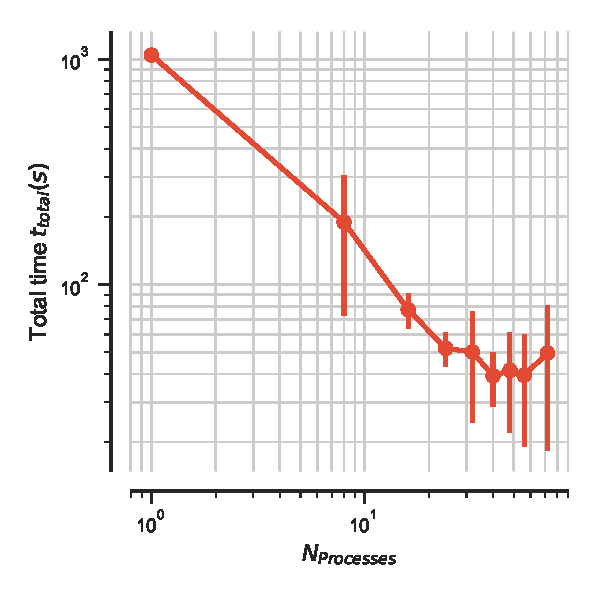
\includegraphics[width=\linewidth]{figures/RMSD-ga4py-t_total.pdf}
  \captionsetup{format=hang}
  \caption{Scaling total}
  \label{fig:MPIscaling-ga4py}
\end{subfigure}
\hfill
\begin{subfigure}{.4\textwidth}
  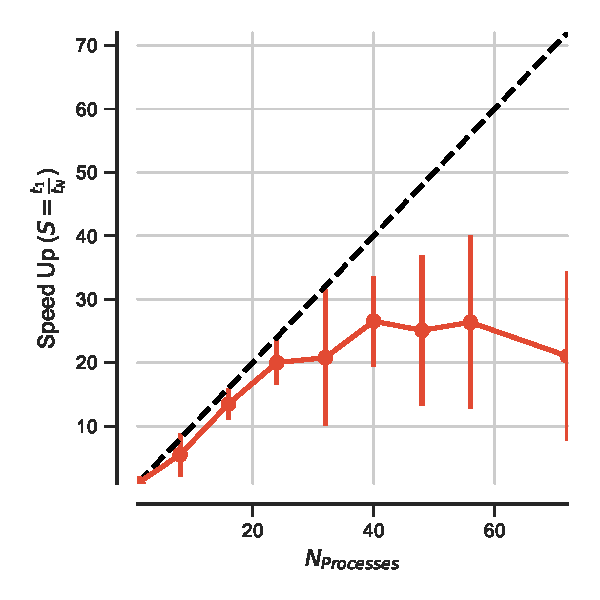
\includegraphics[width=\linewidth]{figures/RMSD-ga4py-speed_up.pdf}
  \captionsetup{format=hang}
  \caption{Speed-up}
  \label{fig:MPIspeedup-ga4py}
\end{subfigure}
\bigskip

\begin{subfigure}{.4\textwidth}
  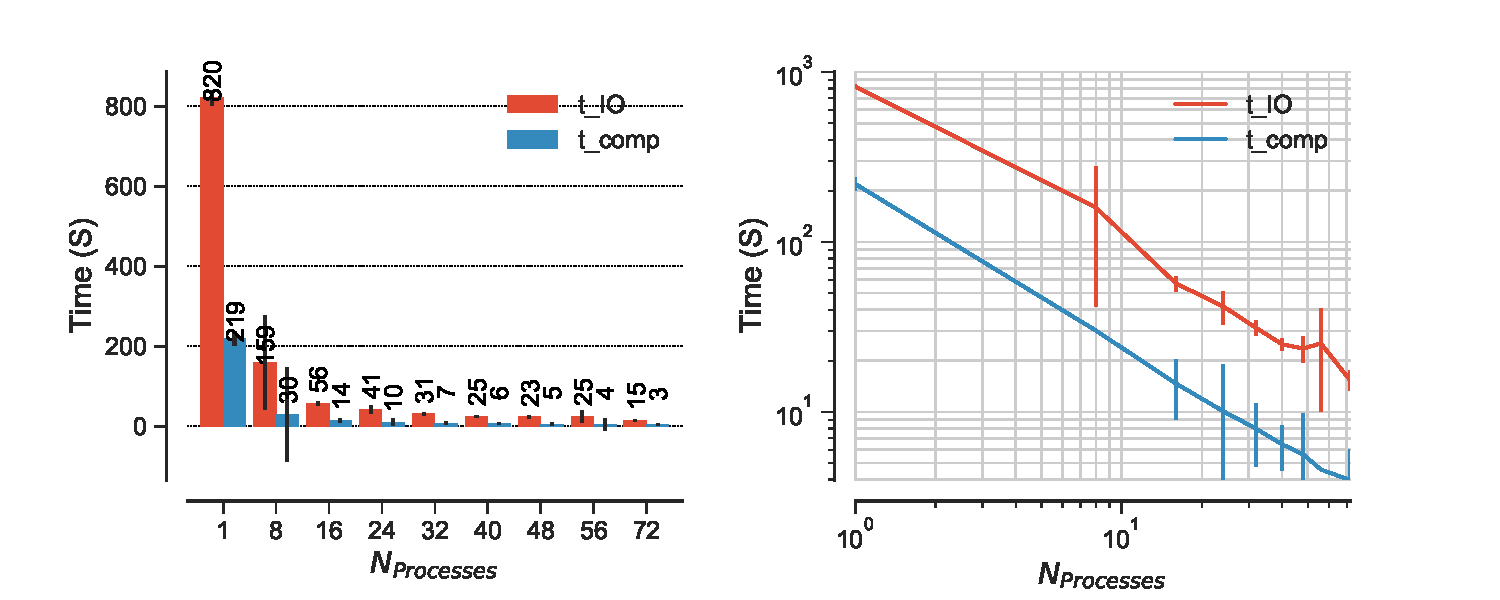
\includegraphics[width=\linewidth]{figures/RMSD-ga4py-time_IO_comparison.pdf}
  \captionsetup{format=hang}
\caption{Scaling for different components}
\label{fig:ScalingComputeIO-ga4py}
\end{subfigure}
\hfill
\begin{subfigure} {.5\textwidth}
  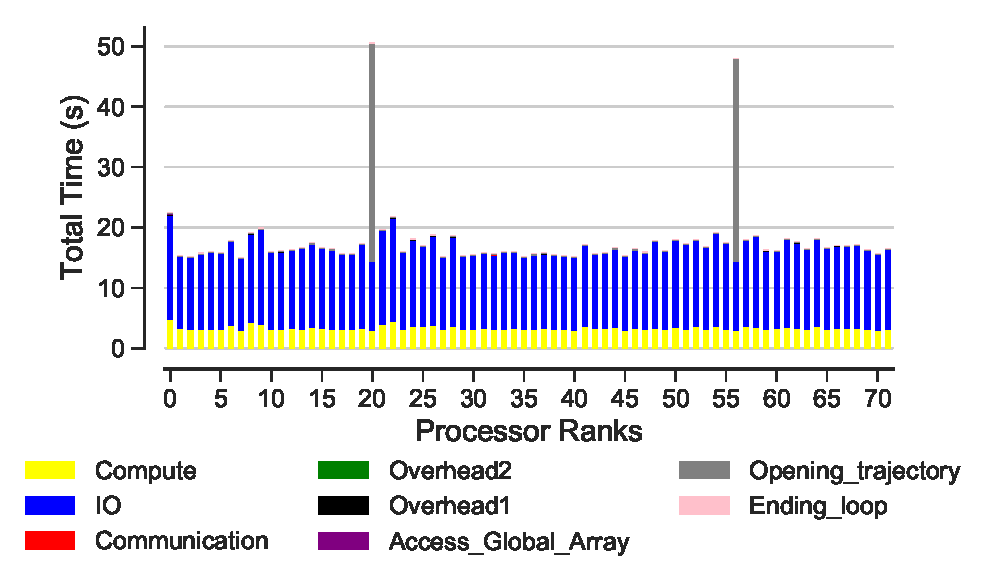
\includegraphics[width=\linewidth]{figures/RMSD-ga4py-BarPlot-rank-comparison_72_1.pdf}
  \captionsetup{format=hang}
  \caption{Time comparison on different parts of the calculations per MPI rank}
  \label{fig:MPIranks-ga4py}
\end{subfigure}

\caption{Performance of the RMSD task with MPI using Global Arrays ($\overline{\tcomp}/\overline{\tIO} \approx 0.3$) on SDSC Comet.
All ranks update the Global Arrays (\texttt{ga\_put()}) and rank 0 accesses the whole RMSD array through the global memory address (\texttt{ga\_get()}).
Five repeats were performed to collect statistics. (a-c) The error bars show standard deviation with respect to mean. 
(d) Compute \tcomp, IO \tIO, communication \tcomm, access to the whole Global Arrays by rank 0, $t_{\text{Access\_Global\_Array}}$, ending the for loop $t_{\text{end\_loop}}$,
  opening the trajectory $t_{\text{opening\_trajectory}}$, and overheads $t_{\text{overhead1}}$, $t_{\text{overhead2}}$ per MPI rank (See Table \ref{tab:notation} for the definition). 
  This is typical data from one run of the 5 repeats. MPI ranks 20 and 56 are stragglers, i.e., 
their total time far exceeds the mean of the all ranks. \textbf{Note:} In serial, there is no communication.}
\label{fig:MPIwithIO-ga4py}
\end{figure}

Motivated by the results in this section, we investigated the influence of the ratio of compute to communication costs ($\overline{\tcomp}/\overline{\tcomm}$) on performance in \ref{sec:tcomm}.
We found evidence to support the hypothesis that a larger ratio was beneficial, provided I/O costs could also be reduced, as discussed in the next section.

\subsection{Reducing I/O Cost}
\label{sec:I/O}
In order to improve performance we needed to employ strategies to avoid the competition over file access across different ranks when the $\overline{\tcomp}/\overline{\tIO}$ ratio was small.
To this end, we experimented with two different ways for reducing the I/O cost:
\begin{inparaenum}[1)]
	\item splitting the trajectory file into as many segments as the number of processes, thus using file-per-process access, and
	\item using the HDF5 file format together with MPI-IO parallel reads instead of the XTC trajectory format.
\end{inparaenum}
We discuss these two approaches and their performance improvements in detail in the following sections.

\subsubsection{Splitting the Trajectories (``subfiling'')}
\label{splitting-traj}
Subfiling is a mechanism previously used for splitting a large multi-dimensional global array to a number of smaller subarrays in which each smaller array is saved in a separate file. Subfiling reduces the file system control overhead by decreasing the number of processes concurrently accessing a shared file~\cite{scalable-IO, scalable-IO1}.
Because subfiling is known to improve programming flexibility and performance of parallel shared-file I/O, we investigated splitting our trajectory file into as many trajectory segments as the number of processes.
The trajectory file was split into $N$ segments, one for each process, with each segment having $N_{b}$ frames. 
This way, each process would access its own trajectory segment file without competing for file accesses. 

\paragraph{Performance with MPI communication}
We ran a benchmark up to 8 nodes (192 cores) and observed rather better scaling behavior with efficiencies above 0.6 (Figure~\ref{fig:MPIscaling-split} and~\ref{fig:MPIspeedup-split}) with the delay time for stragglers reduced from $65sec$ to about $10sec$ for 72 processes. 
However, scaling is still far from ideal due to communication (using MPI). 
Although the delay due to communication was much smaller as compared to parallel RMSD with shared-file I/O (compare Figure~\ref{fig:MPIranks-split} ($\tcomm^{\text{Straggler}} \gg \tcomp+\tIO$) to Figure~\ref{fig:MPIranks} ($\tcomm^{\text{Straggler}} \approx \tcomp+\tIO$)), it is still delaying several processes and resulted in longer job completion times (Figure~\ref{fig:MPIranks-split}). 
These delayed tasks impacted performance so that speed-up remained far from ideal (Figure~\ref{fig:MPIspeedup-split}).

\begin{figure}[ht!]
\centering
\begin{subfigure}{.32\textwidth}
  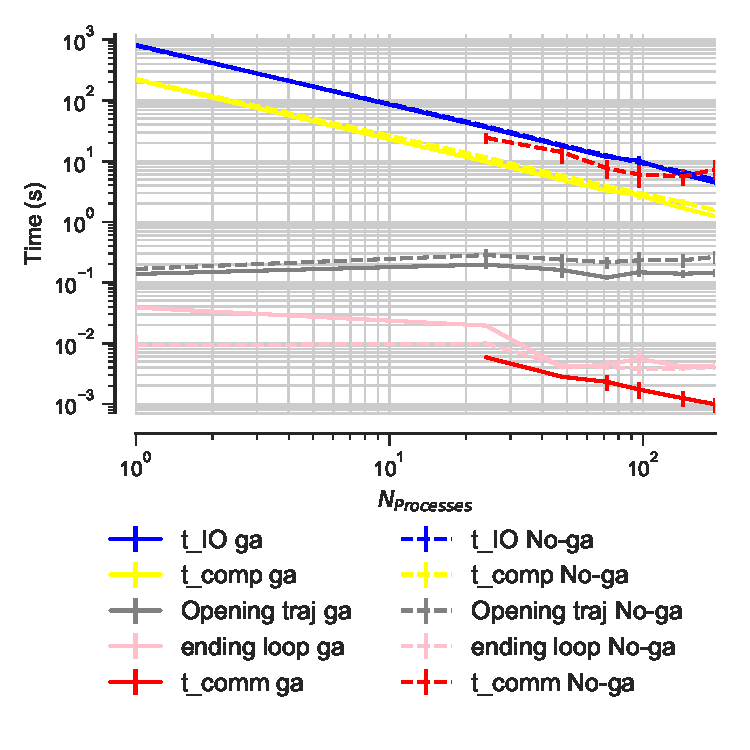
\includegraphics[width=\linewidth]{figures/Comparison_IO_compute_scaling_traj_splitting.pdf}
  \captionsetup{format=hang}
  \caption{Scaling for different components}
  \label{fig:ScalingComputeIO-split}
\end{subfigure}
\hfill
\begin{subfigure}{.3\textwidth}
  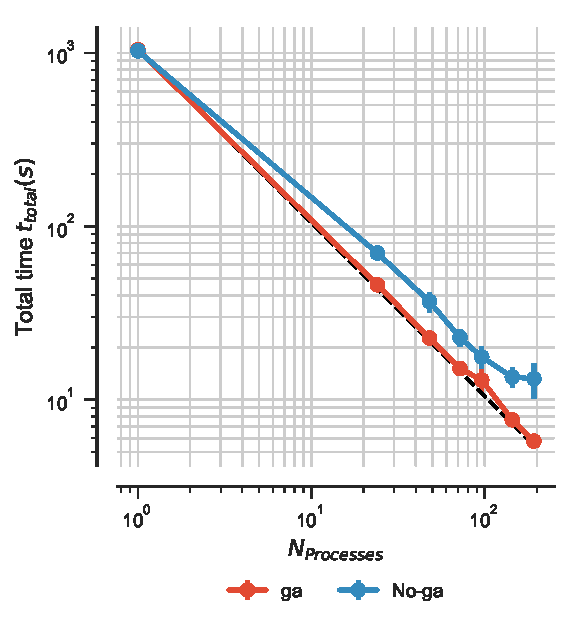
\includegraphics[width=\linewidth]{figures/Comparison_tot_time_traj_splitting.pdf}
  \caption{Scaling total}
  \label{fig:MPIscaling-split}
\end{subfigure}
\hfill
\begin{subfigure}{.3\textwidth}
  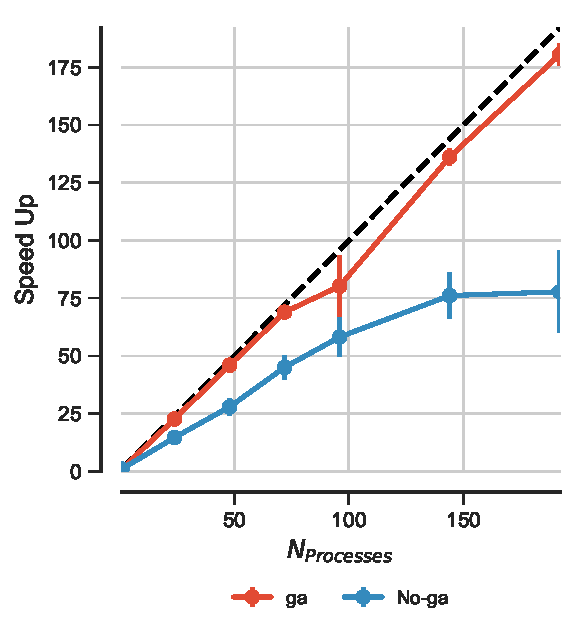
\includegraphics[width=\linewidth]{figures/Comparison_Speed_UP_traj_splitting.pdf}
  \captionsetup{format=hang}
  \caption{Speed-up}
  \label{fig:MPIspeedup-split}
\end{subfigure}
\bigskip

\begin{subfigure} {.45\textwidth}
  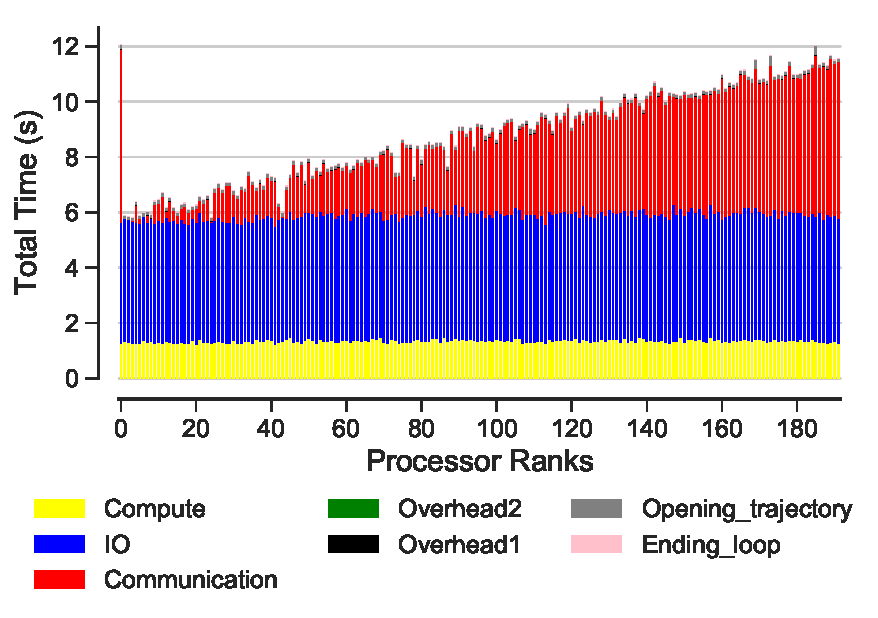
\includegraphics[width=\linewidth]{figures/split-BarPlot-rank-comparison_192_5.pdf}
  \captionsetup{format=hang}
   \caption{Time comparison on different parts of the calculations per MPI rank without Global Arrays}
  \label{fig:MPIranks-split}
\end{subfigure}
\hfill
\begin{subfigure} {.5\textwidth}
  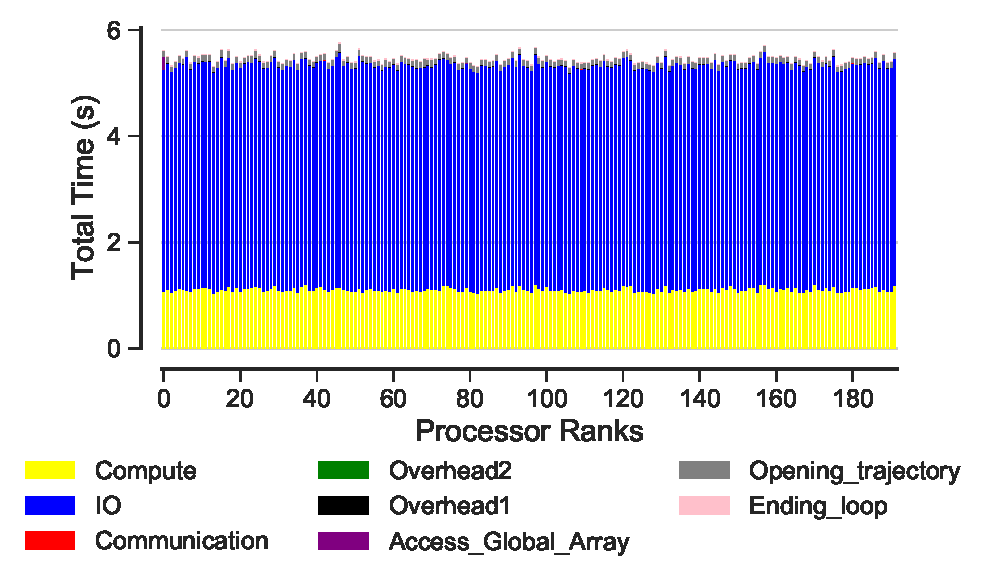
\includegraphics[width=\linewidth]{figures/split-ga-BarPlot-rank-comparison_192_5.pdf}
  \captionsetup{format=hang}
  \caption{Time comparison on different parts of the calculations per MPI rank using Global Arrays}
  \label{fig:MPIranks-split-ga}
\end{subfigure}

\caption{Comparison on the performance of the RMSD task ($\overline{\tcomp}/\overline{\tIO} \approx 0.3$) on \emph{SDSC Comet} when the trajectories are split. For communicating the results, either Global Arrays (``ga'') or MPI (no Global Arrays, ``No-ga'') was used.  In the case of Global Arrays, all ranks updates the Global Arrays (\texttt{ga\_put()}) and rank 0 accessed the whole RMSD array through the global memory address (\texttt{ga\_get()}).  Five repeats were performed to collect statistics. (a) Compute and I/O scaling versus number of processes (b) Total time scaling versus number of processes (c) Speed-up (a-c) The error bars show standard deviation with respect to mean. (d-e) Compute \tcomp, IO \tIO, communication \tcomm, access to the whole Global Arrays by rank 0, $t_{\text{Access\_Global\_Array}}$, ending the for loop $t_{\text{end\_loop}}$, opening the trajectory $t_{\text{opening\_trajectory}}$, and overheads $t_{\text{overhead1}}$, $t_{\text{overhead2}}$ per MPI rank (see Table \ref{tab:notation} for the definitions). When Global Arrays was not used, the performance was decreased due to the non-uniform communication time across different ranks. However, with Global Arrays communication time was significantly reduced and scaling was close to ideal. \textbf{Note:} In serial, there is no communication.}
\label{fig:MPIwithIO-split}
\end{figure}

\paragraph{Performance using Global Arrays}
In Section~\ref{Global-Array} we showed that Global Arrays substantially reduced the communication cost. 
We wanted to quantify the performance when splitting the trajectory file while using Global Arrays.
Under otherwise identical conditions as in the previous section we now observed near ideal scaling behavior with efficiencies above 0.9 (Figure~\ref{fig:MPIscaling-split} and~\ref{fig:MPIspeedup-split}) without any straggler tasks (Figure~\ref{fig:MPIranks-split-ga}).
Although the reason why in our case Global Arrays appeared to be more efficient than direct MPI-based communication remains unclear, these results showed that contention for file access clearly impacted performance. By removing the contention, near ideal scaling could be achieved.

\paragraph{Further considerations for splitting trajectories}
The subfiling approach appears promising but it requires preprocessing of trajectory files and additional storage space for the segments.
We benchmarked the necessary time for splitting the trajectory using different number of MPI processes (Table~\ref{tab:timing-splitting}).
These preprocessing times were not included in the estimates because we are focusing on better understanding the principle causes of stragglers and we wanted to make the results directly comparable to the results of the previous sections.
Nevertheless, from an end user perspective, preprocessing of trajectories can be integrated in workflows (especially as the data in Table~\ref{tab:timing-splitting} indicate good scaling) and the preprocessing time can be quickly amortized if the trajectories are analyzed repeatedly.

Often trajectories from MD simulations on HPC machines are produced and kept in small chunks that would need to be concatenated to form a trajectory but that might be useful for the subfiling approach.
However, it might not be feasible to have exactly one trajectory segment per MPI rank.
In~\ref{sec:chainreader} we investigated if existing functionality in MDAnalysis that can create virtual trajectories from trajectory segments could benefit from the subfiling approach.
We found some improvements in performance but discovered limitations in the design that first have to be overcome before equivalent performance can be reached.
 
\subsubsection{MPI-based Parallel HDF5}
\label{HDF5}
Another approach we examined to improve I/O scaling was MPI-based Parallel HDF5. 
We converted our XTC trajectory file into a simple custom HDF5 format so that we could test the performance of parallel I/O with the HDF5 file format.
The code for this file format conversion can be found in the GitHub repository.
The time it took to convert our XTC file with $2,512,200$ frames into HDF5 format was about $5,400sec$ on a local workstation with network file system (NFS).

We ran our benchmark on up to 16 nodes (384 cores) and we observed near ideal scaling behavior with parallel efficiencies above 0.8 up to 8 nodes (Figure~\ref{fig:comparison_efficiency} and Figures~\ref{fig:MPIscaling-hdf5} and~\ref{fig:MPIspeedup-hdf5}) with no straggler tasks (Figure~\ref{fig:MPIranks-hdf5}).
The trajectory reading I/O (\tIO) was the dominant contribution, followed by compute (\tcomp), but because both contributions scaled well, overall scaling performance remained good, even for 384 cores.
We observed a low-performing outlier for 12 nodes (288 cores) with slower I/O than typical but did not further investigate.
Importantly, the trajectory opening cost remained negligible (in the millisecond range) and the cost for MPI communication also remained small (below 0.1 s, even for 16 nodes).
Overall, parallel MPI with HDF5 appears to be a robust approach to obtain good scaling, even for I/O-bound tasks.

\begin{figure}[ht!]
\centering
\begin{subfigure}{.4\textwidth}
  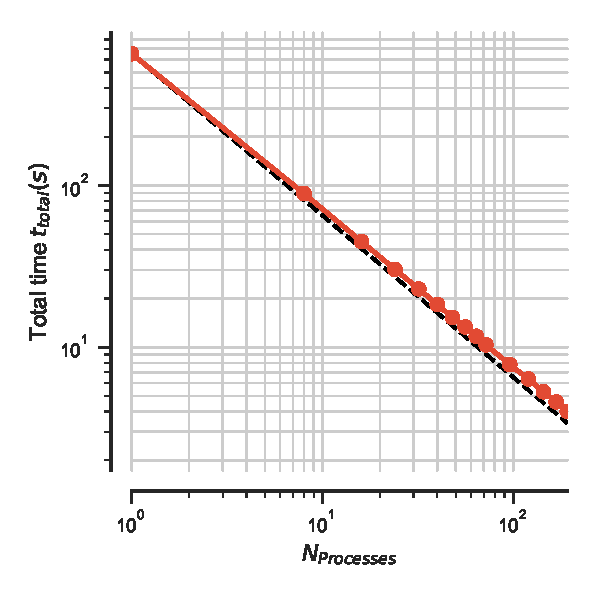
\includegraphics[width=\linewidth]{figures/hdf5-t_total.pdf}
  \caption{Scaling total}
  \label{fig:MPIscaling-hdf5}
\end{subfigure}
\hfill
\begin{subfigure}{.4\textwidth}
  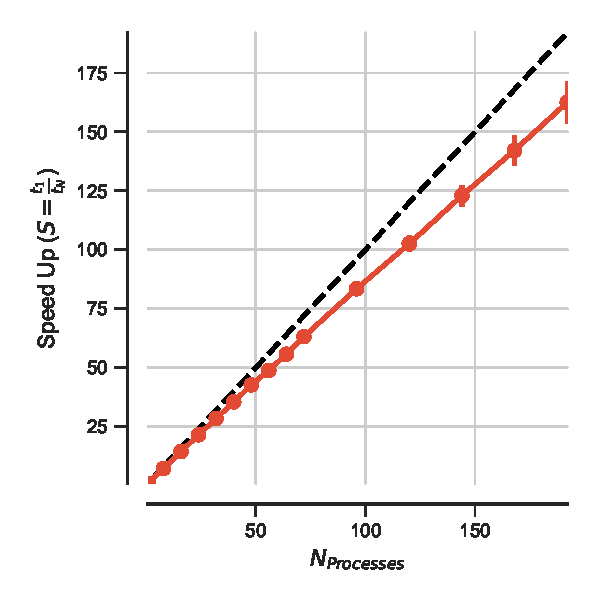
\includegraphics[width=\linewidth]{figures/hdf5-speed_up.pdf}
  \caption{Speed-up}
  \label{fig:MPIspeedup-hdf5}
\end{subfigure}
\bigskip

\begin{subfigure}{.4\textwidth}
\centering
  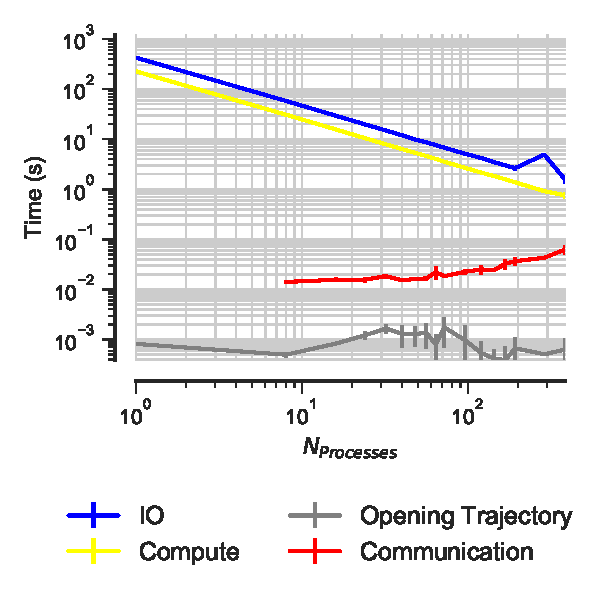
\includegraphics[width=\linewidth]{figures/hdf5-time_comp_IO_comparison.pdf}
  \captionsetup{format=hang}
\caption{Scaling for different components}
\label{fig:ScalingComputeIO-hdf5}
\end{subfigure}
\hfill
\begin{subfigure} {.5\textwidth}
  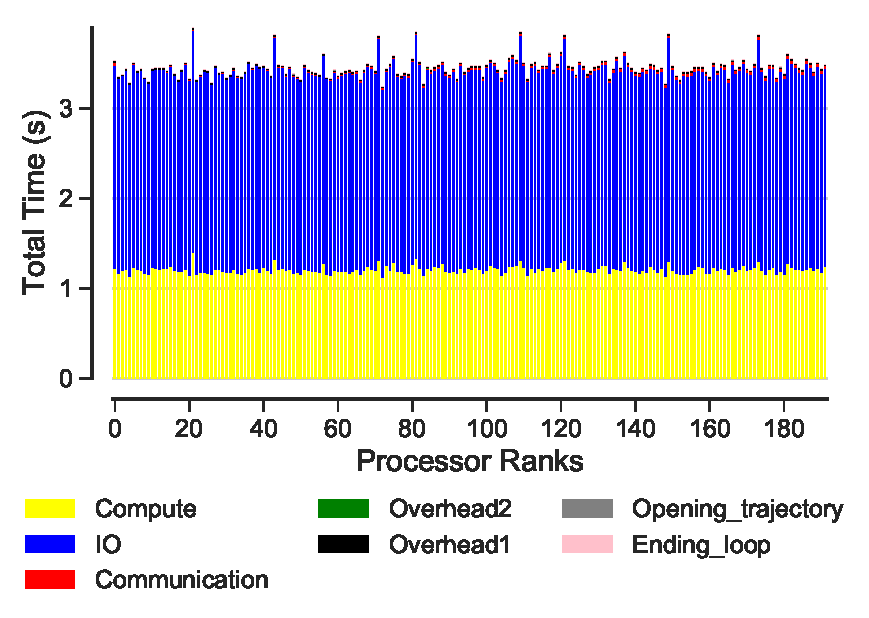
\includegraphics[width=\linewidth]{figures/hdf5-BarPlot-rank-comparison_192_4.pdf}
  \captionsetup{format=hang}
  \caption{Time comparison on different parts of the calculations per MPI rank}
  \label{fig:MPIranks-hdf5}
\end{subfigure}
%
\caption{Performance of the RMSD task with MPI-based parallel HDF5 ($\overline{\tcomp}/\overline{\tIO} \approx 0.3$) on SDSC Comet.
Data are read from the file system from a shared HDF5 file format instead of XTC format (Independent I/O) and results are communicated back to rank 0 (communications included). 
Five repeats were performed to collect statistics. (a-c) The error bars show standard deviation with respect to mean. (d) Compute \tcomp, IO \tIO, communication \tcomm, ending the for loop $t_{\text{end\_loop}}$,
  opening the trajectory $t_{\text{opening\_trajectory}}$, and overheads $t_{\text{overhead1}}$, $t_{\text{overhead2}}$ per MPI rank (See Table \ref{tab:notation} for the definition).
  This is typical data from one run of the 5 repeats. No straggler is observed. \textbf{Note:} In serial, there is no communication. I am reporting the slowest rank per timing, and that is averaged over all repeats.}
\label{fig:MPIwithIO-hdf5}
\end{figure}

\subsection{Likely Causes of Stragglers}
\label{sec:likelycauses}
The data indicated that increases in the duration of both MPI communication and trajectory file access lead to large variability in the run time of individual MPI processes and ultimately poor scaling performance beyond a single node.
A discussion of likely causes for stragglers begins with the observation that opening and reading a single trajectory file from multiple MPI processes appeared to be at the center of the problem. 

In MDAnalysis, individual trajectory frames are loaded into memory, which ensures that even systems with tens of millions of atoms can be efficiently analyzed on resources with moderate RAM sizes.
The test trajectory (file size 30 GB) had $2,512,200$ frames in total so each frame was about 0.011 MB in size.
With $\tIO \approx 0.3~\text{ms}$ per frame, the data were ingested at a rate of about $40$~MB/s for a single process.
For 24 MPI ranks (one \emph{SDSC Comet} node), the aggregated reading rate would have been about 1 GB/s.
Although, such a value seemed to be well within the available bandwidth of 56 Gb/s of the Infini-band network interface that served the Lustre file system, in practice the aggregated I/O bandwidth for reading from a shared file was actually fairly small which was expected based on the studies in~\cite{ATPESC2016}.
Furthermore, in our study the default Lustre stripe size value was 1~MB, i.e., the amount of contiguous data stored on a single Lustre object storage target (OST).
Each I/O request read a single Lustre stripe but because the I/O size (0.011~MB) was smaller than the stripe size, many of these I/O requests were likely just accessing the same stripe on the same OST but nevertheless had to acquire a new reading lock for each request.

The reason for this behavior is related to ensuring POSIX consistency that relates to POSIX I/O API and POSIX I/O semantics, which can have adverse effects on scalability and performance.
Parallel file systems like Lustre implement sophisticated distributed locking mechanisms to ensure consistency.
For example, locking mechanisms ensures that a node can not read from a file or part of a file while it might be being modified by another node. 
In fact, when the application I/O is not designed in a way to avoid scenarios where multiple nodes are fighting over locks for overlapping extents, Lustre can suffer from scalability limitations~\cite{optimize_lustre}.
Continuously keeping metadata updated in order to have fully consistent reads and writes (POSIX metadata management), requires writing a new value for the file's last-accessed time (POSIX atime) every time a file is read, imposing a significant burden on parallel file system~\cite{POSIX2017}. 

It was observed that contention for the interconnect between OSTs and compute nodes due to MPI communication may lead to variable performance in I/O measurements~\cite{Mache:2005aa}.
Conversely, our data suggest that single-shared-file I/O on Lustre can negatively affect MPI communication as well, even at moderate numbers (tens to hundreds) of concurrent requests, similar to recent network simulations that predicted interference between MPI and I/O traffic~\cite{Brown:2018ab}.
This work indicated that MPI traffic (inter-process communication) can be affected by increasing I/O, and in particular, a few MPI processes were always delayed by 1-2 orders of magnitude more than the median time.
Thus, suggesting that our observed stragglers with large variance in the MPI communication might be due to interference with the I/O requests on the same network.

